%The present analysis was completed using an \textit{art::EDAnalyzer} module and a 
This analysis uses a series of sequential cuts to identify neutrino candidates and exclude cosmic backgrounds by leveraging information derived from the Pandora reconstruction~\cite{acciarri2018pandora}. Furthermore, the beam information was studied in conjunction with the detector activity, utilizing the number of TPs contained in Time Slice objects.

\subsection{H4 and H6 beamline monitoring} \label{chap:anaBeamMonitoring}
%As outlined in sections \ref{sec:SPSspill} and \ref{sec:beam_monitoring}, 
The PD-HD response was analyzed for each beam configuration (Table \ref{tab:data_table}) in combination with the beam monitors accessed through TIMBER. Consequently, the number of TPs contained within a one-second Time Slice was represented throughout the runtime (Figure \ref{fig:tp_over_time}). This representation always took into account the spill mode, as determined by the PoT values, and the threshold of $10^{12}$ protons on target. In this manner, any TP excess in the detector coming from the secondary-beam activity can be distinguished from the baseline TP rate when the beam spill is turned off, close to 2 million TPs per second.
% Finally, to discern the trend, the scintillation counts used to correlate the beamline activity with the detector response were scaled to the same order of magnitude as the PoT values.

\begin{figure}[!hb]
    \centering
    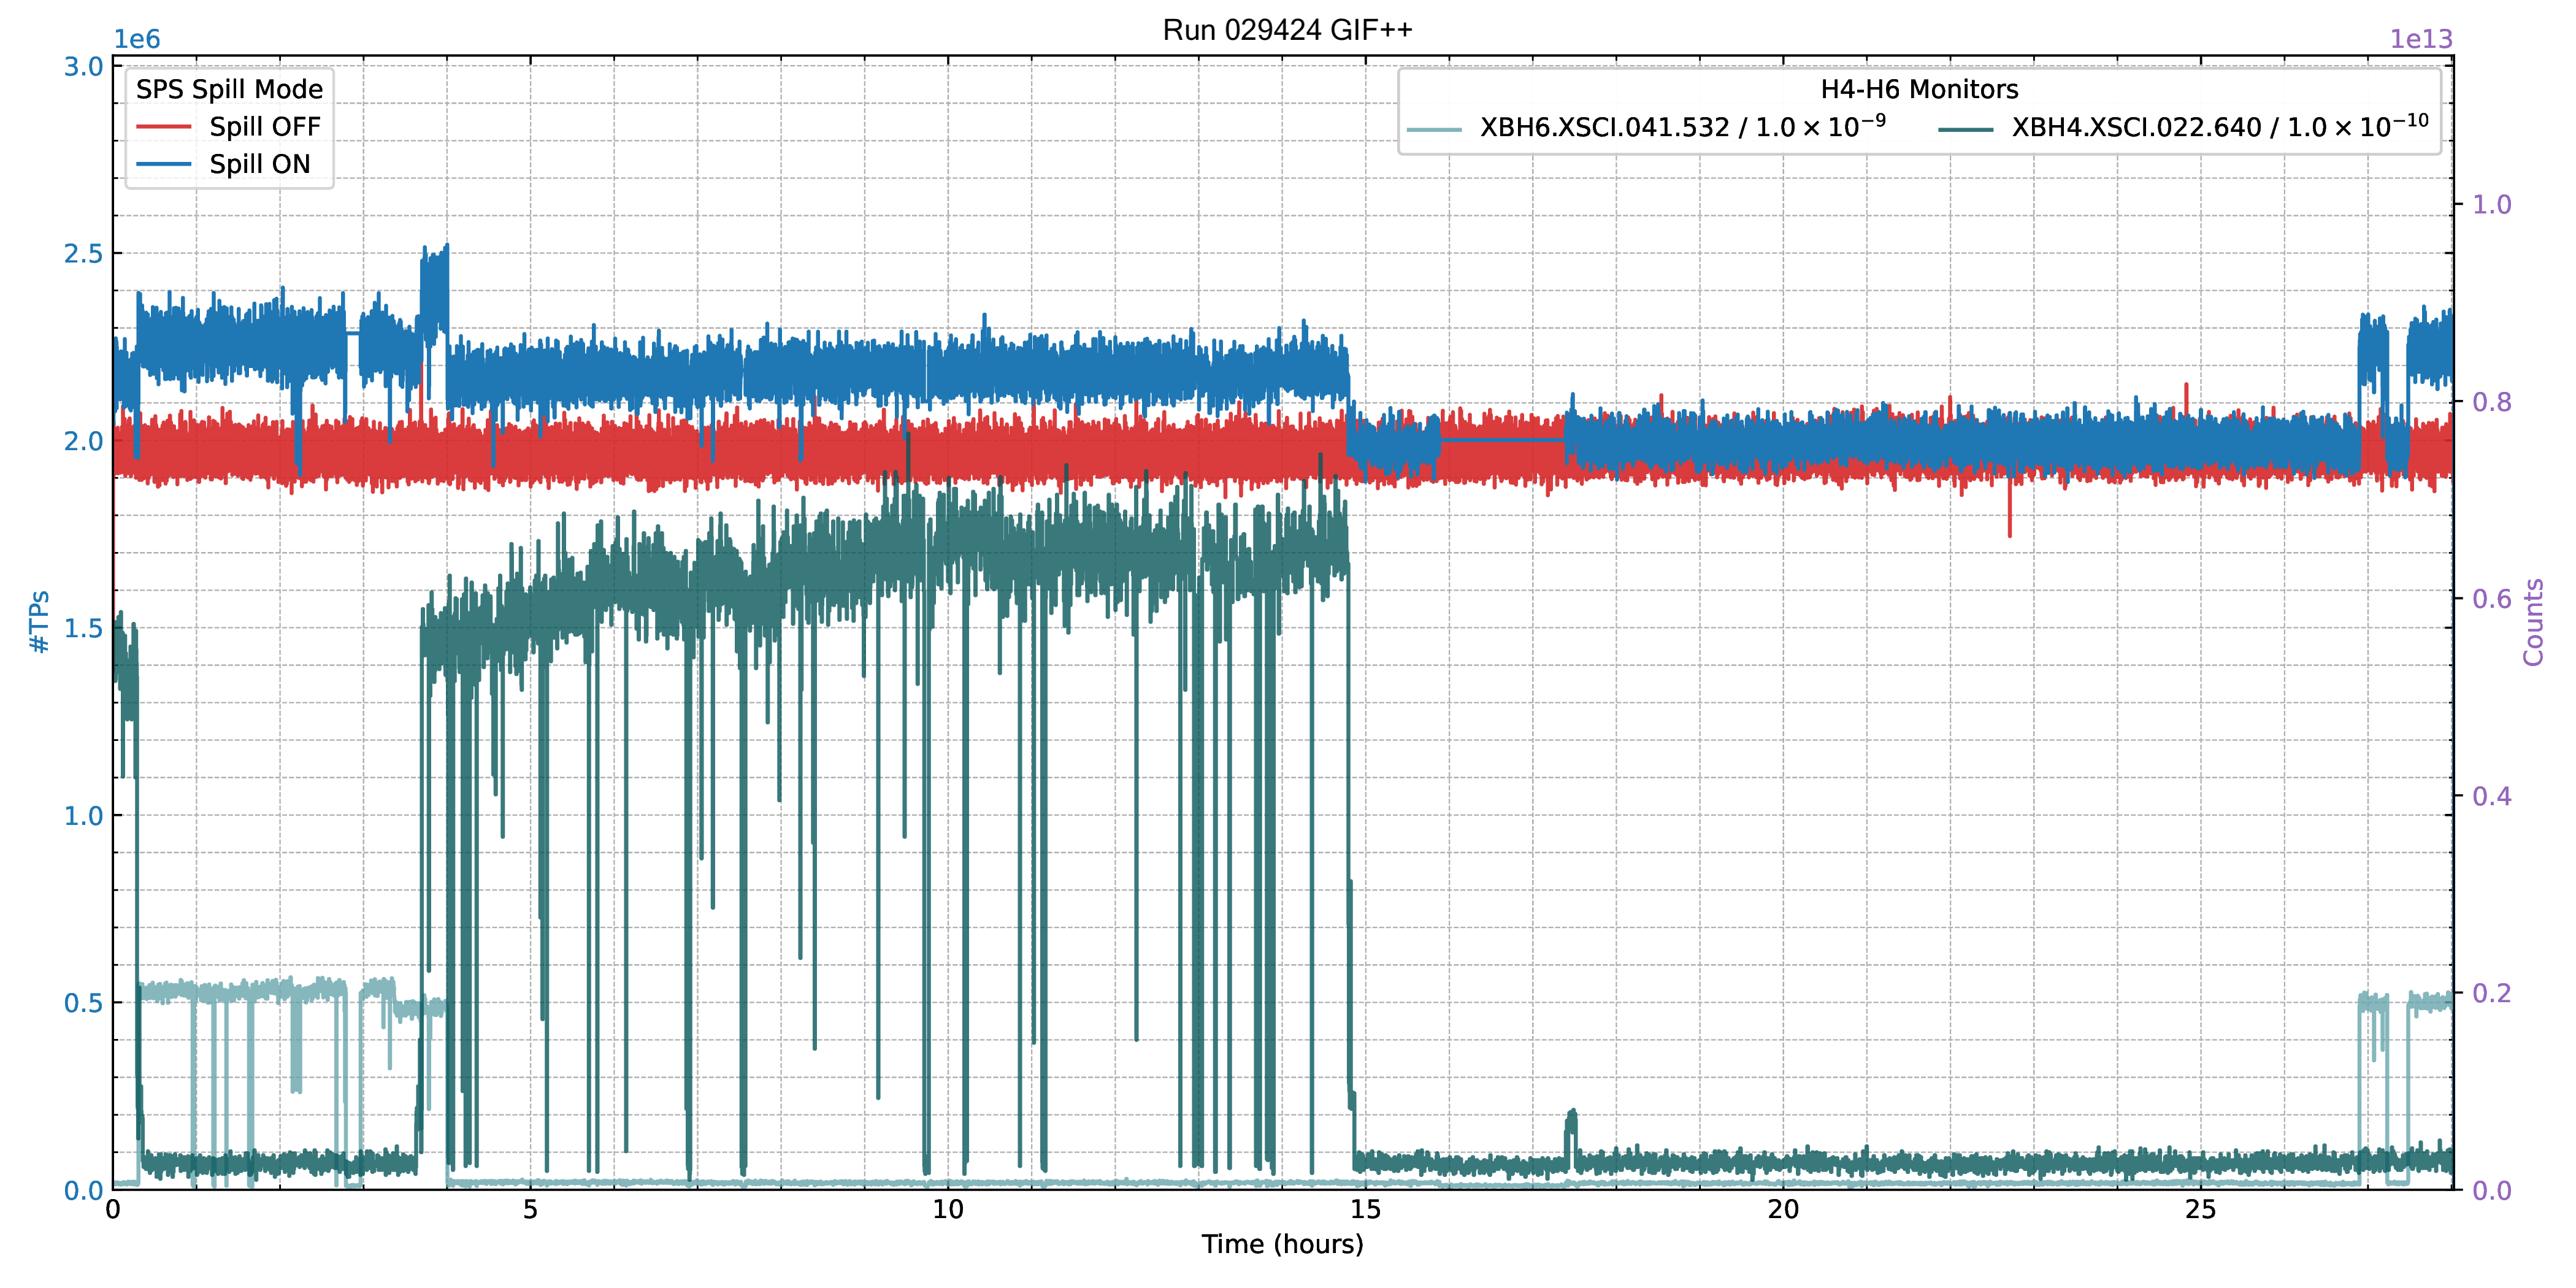
\includegraphics[width=0.85\linewidth]{sections/analysis/TPdistribution/run029424_H4H6_step.png}\\
    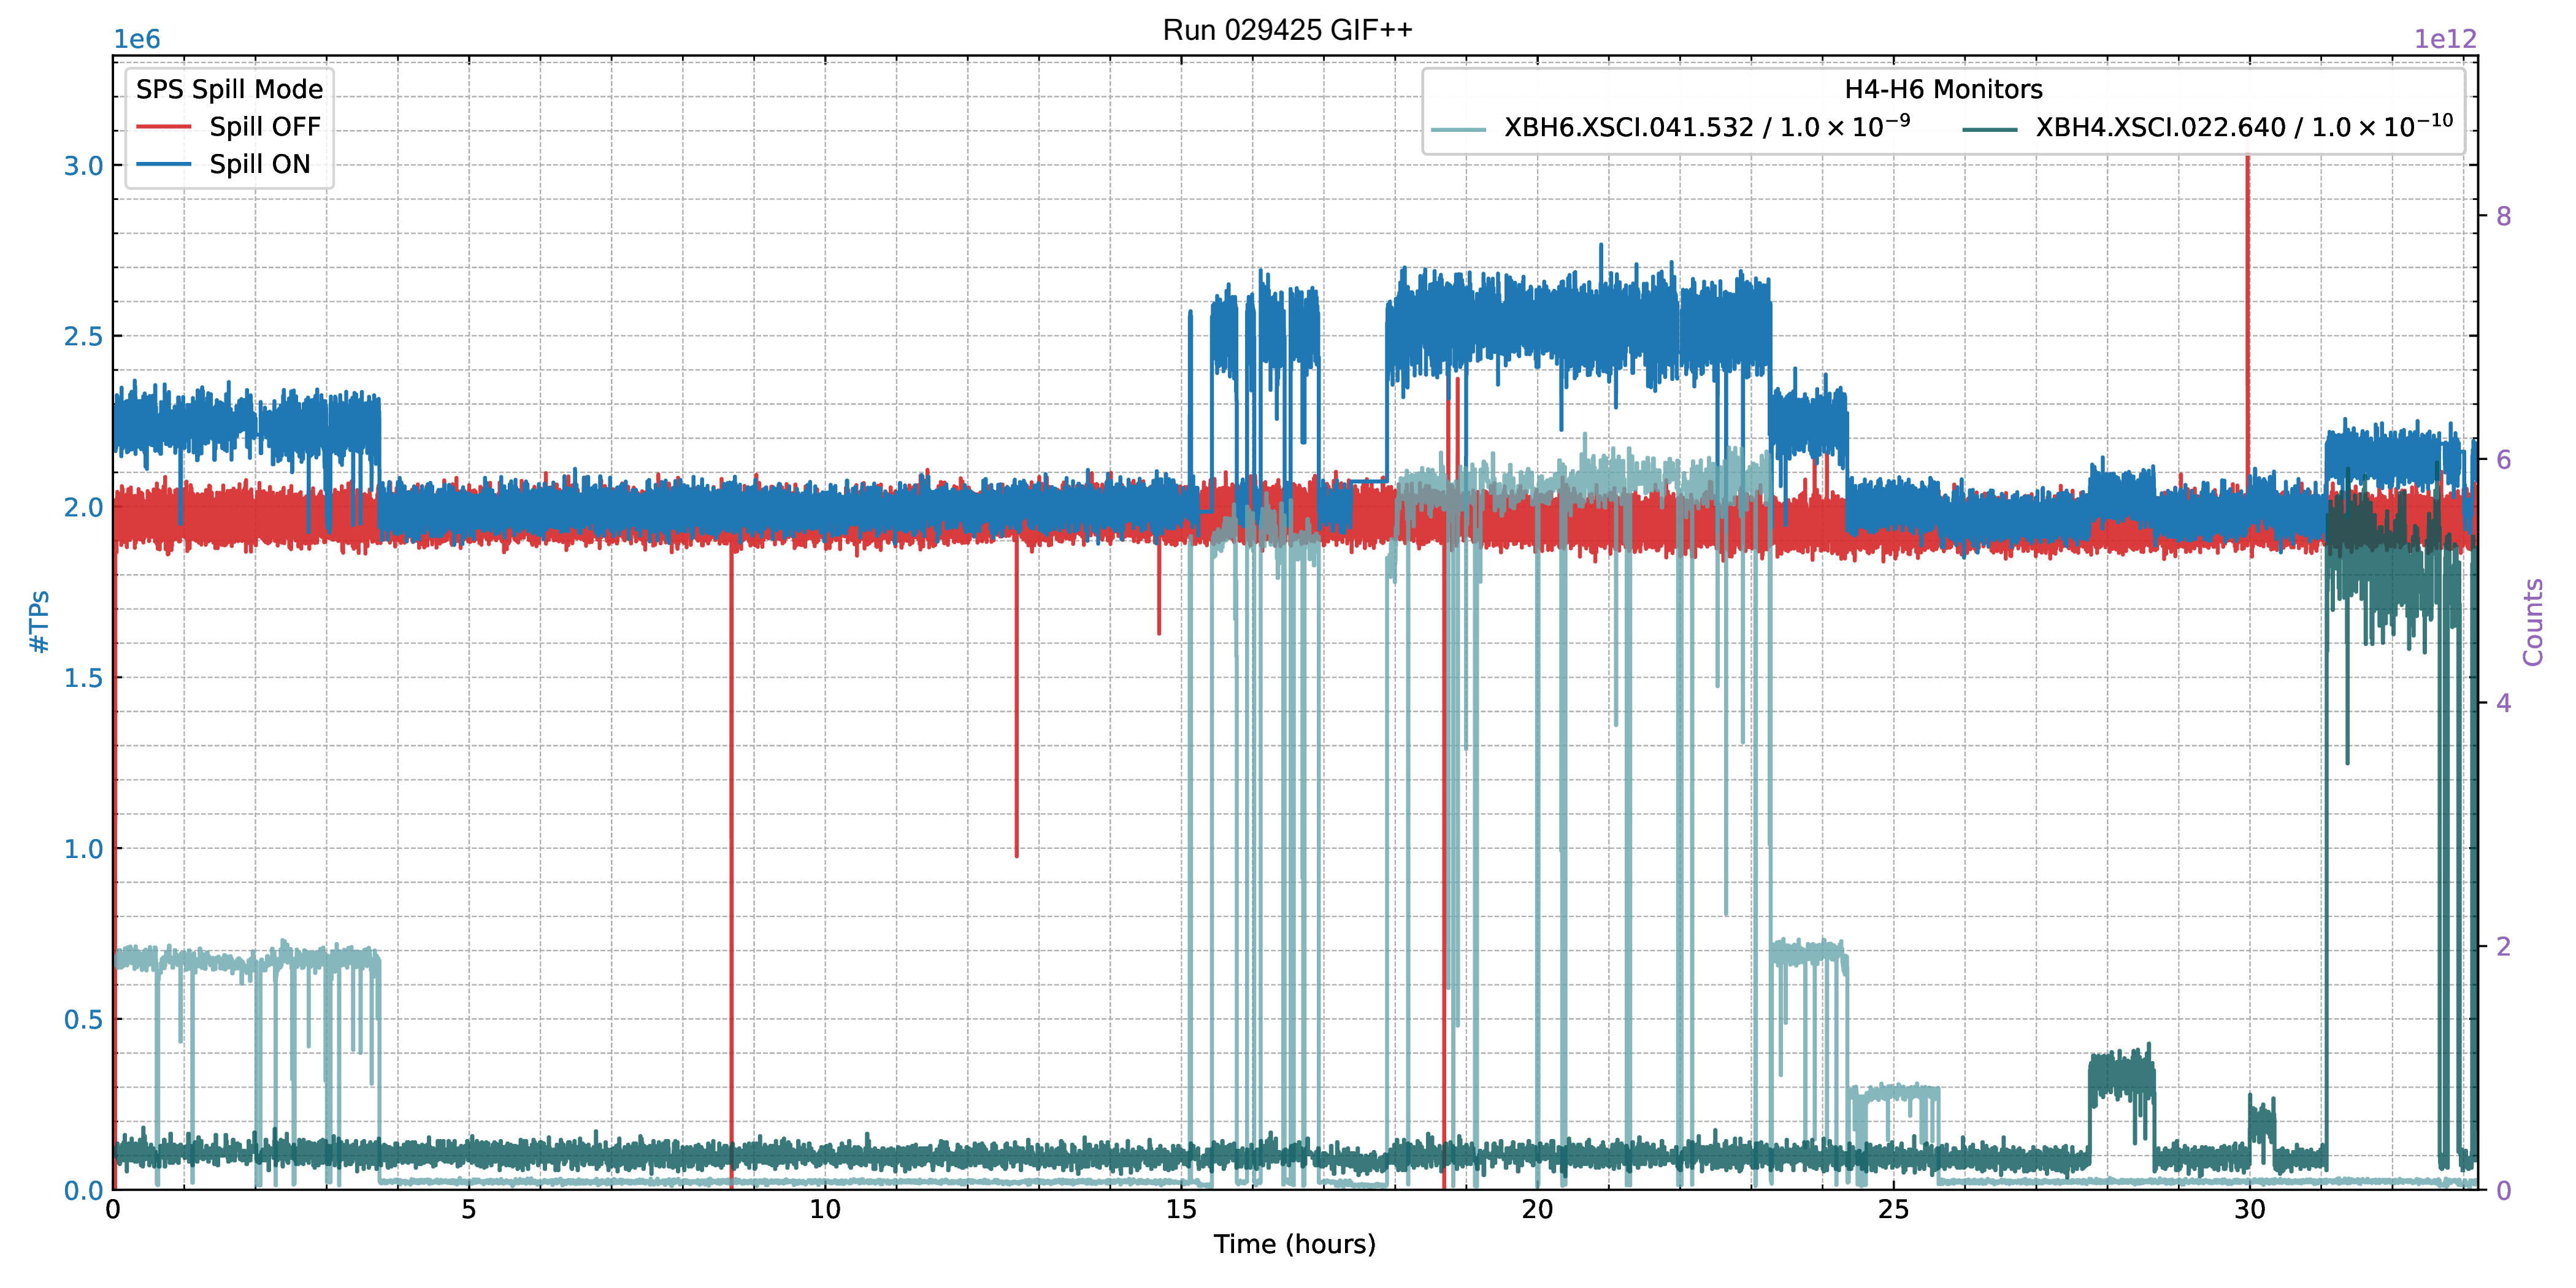
\includegraphics[width=0.85\linewidth]{sections/analysis/TPdistribution/run029425_H4H6_step.png}\\
    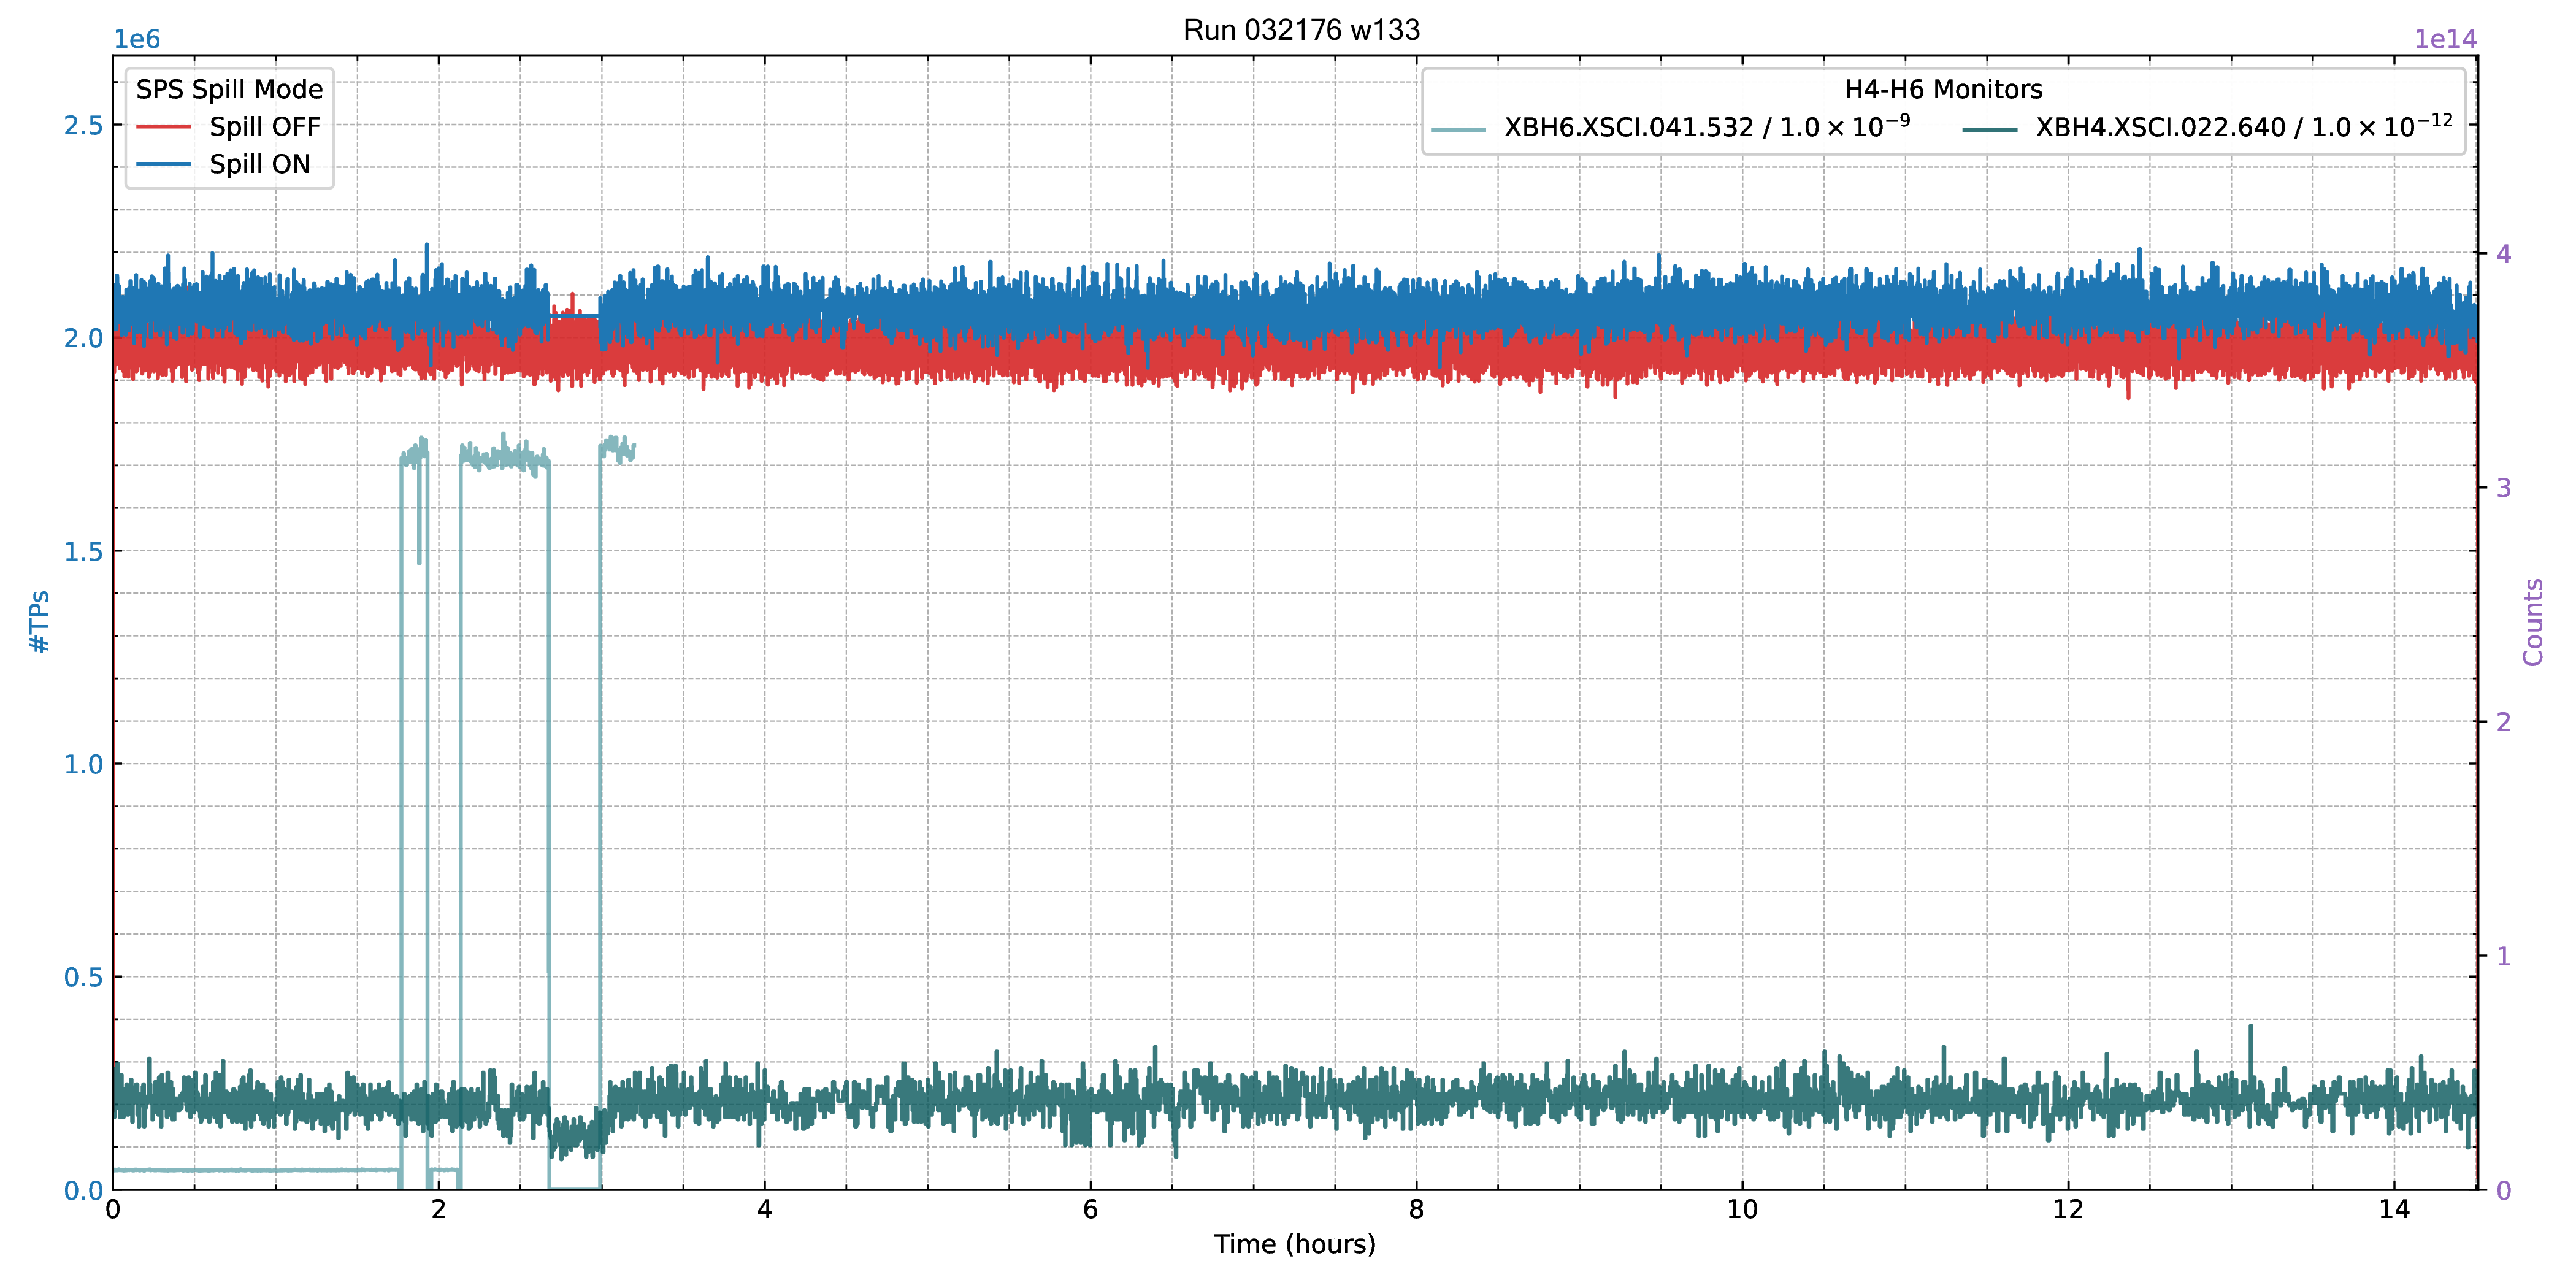
\includegraphics[width=0.85\linewidth]{sections/analysis/TPdistribution/run032176_H4H6_step.png}
    \caption{Trigger primitive distribution per second for SPS spill mode On (blue) and Off (red). The closest scintillation counters to PD-HD, which are related to the H4 and H6 beamlines, are also included in the graphs. The noticeable excess of spill-on TPs is explained by the H4 and H6 beamline activity.}
    \label{fig:tp_over_time}
\end{figure}

%Even for comparable PoT intensity, 
There are time intervals during which the number of TPs remains constant during both spill-on (blue histogram) and spill-off (red histogram) periods. Conversely, for the GIF++ configuration there are other times when there are distinct regions above the baseline during the spill. This excess, which exhibits a fairly good correlation with the activity registered by H4 and H6 counters, is attributed to other beam-induced particles that are recorded in the detector but are not accounted for in the simulations. In the W133 configuration, the excess of spill-on TPs was uniform and modest compared to the baseline. Neither a significant excess of TPs nor clear correlations with the beamline activity were observed during the various runs.
%However, neutrinos from secondary beams are expected to be less energetic and not triggered, as depicted in Figure \ref{fig:MC_trigger_efficiency}. To shed light on the neutrino energy distribution resulting from beam-induced particles, the muon-momentum distribution analysis for the GIF++ configuration is underway, together with the three-body decay system. %\textcolor{blue}{Add study here once completed.}

Initially, to ensure the robustness of the analysis, only the time periods without a noticeable increase in the TP rate beyond the baseline due to the beamline activity, are considered in these studies. Additionally, time intervals with extra TP activity will eventually be included. %for the sake of triggered-neutrino contributions from beam-induced particles.

% To further explore this, the TP distribution, as well as the linear correlations between the spill-on TPs, and the diverse set of H4 scintillation counters are depicted in Figure \ref{fig:tp_sci_correlations}. This is carried out for runs 29424 and 29918, where correlations were observed, as elucidated in section \ref{sec:beam_monitoring}. For run 29424, under the wobbling GIF++ configuration, we clearly observe two distributions related to the TPs recorded when the SPS spill was turned on, as reflected in Figure \ref{fig:tp_over_time}. In contrast, for run 29918, recorded with the magnet w133 configuration, we only observe one distribution when the spill was on. Regarding the correlations, they range between 0.45 and 0.60 overall. Additional statistics being recorded during trigger tests in PD-VD will provide conclusive evidence.

% \begin{figure}[!h]
%     \centering
%     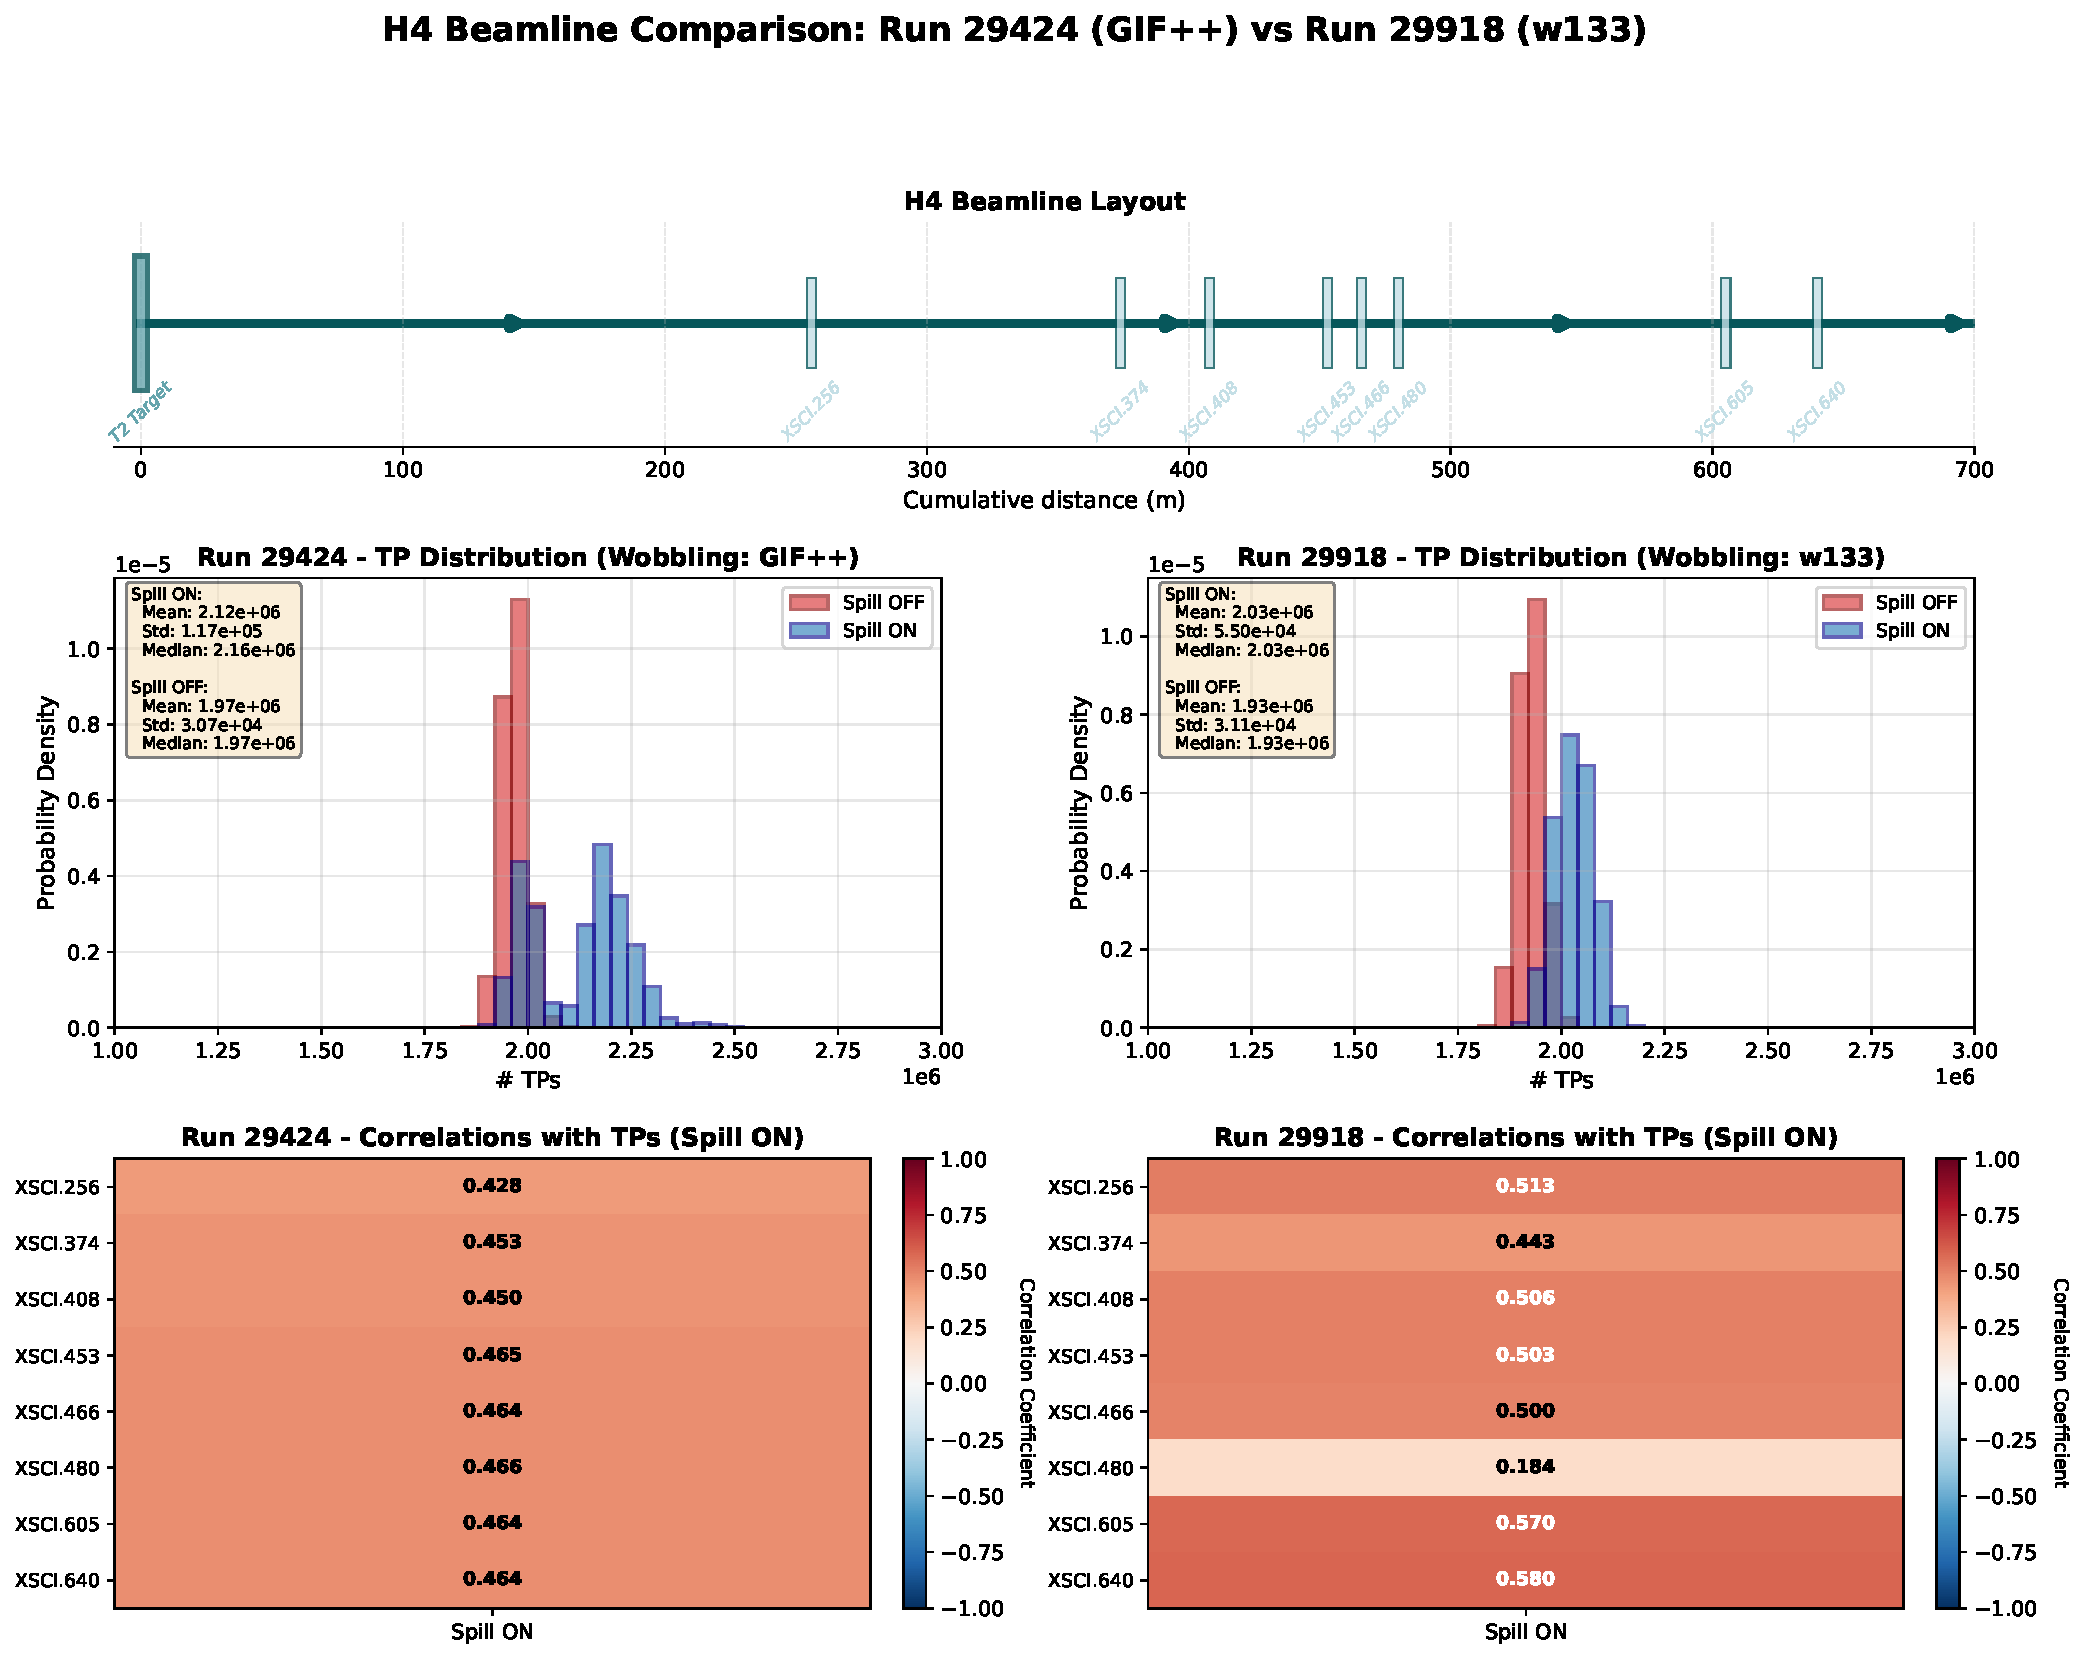
\includegraphics[width=1\linewidth]{sections/analysis/TPdistribution/run_29424_vs_29918_with_beamline.pdf}
%     \caption{Normalized TP distributions and linear correlation matrices between the PD-HD activity, through the number of TPs, and the set of scintillation counters distributed along the H4 beamline. They are tagged by the cumulative distance, in meters, from the T2 target, as indicated by the H4 beamline layout at the top. This is accounted for the runs showing correlations: runs 29924 and 29918.}
%     \label{fig:tp_sci_correlations}
% \end{figure}

\subsection{Analysis software framework} \label{chap:anaValidation}
% LArSoft is a shared software framework for simulation, reconstruction, and analysis of liquid-argon time projection chamber experiments. In the LArSoft workflow, an art analyzer is a user-created and configurable module that performs specific analysis tasks on reconstructed and/or simulated data. Specifically, it refers to a C++ module executed for each event in a LArSoft job. Its primary function is to read the output of producer modules, which generate data, and perform specific analysis operations on it. These operations includes:
% \begin{itemize}
%     \item Reading reconstructed objects, such as tracks and showers.
%     \item Creating plots and histograms of various physical quantities.
%     \item Calculating new variables or metrics.
%     \item Saving results to a ROOT file, a widely used data format in particle physics.
% \end{itemize}
% In essence, an art analisys module is a customizable tool that enables users to explore simulated or reconstructed data to extract the physics results they seek. The strategy employed for this search involves utilizing an art analyzer to extract information from the reconstructed files and perform potentially intricate operations on the data. Thereafter, the processed values are output in a plain ROOT file, which can be utilized for selection, plotting, and significance calculation in a separate code.
In the LArSoft workflow, an art analyzer is a user-created and configurable module that performs specific analysis tasks on reconstructed and/or simulated data. Specifically, it refers to a C++ module executed for each event in a LArSoft job. A key aspect is the validation of the art analyzer modules responsible for selecting reconstructed neutrino data in PD-HD. This validation process is conducted using a small Monte Carlo production. To achieve this, reconstructed properties obtained from the algorithm are compared with the true Monte Carlo information. The strategy employed is straightforward: the true information is contrasted with the outcome from primary Pandora neutrinos within the most energetic slice. Pandora slices consist of topologically distinct collections of hits categorized based on proximity and pointing information. Each slice should contain a single, distinct neutrino interaction or cosmic-ray.

% To achieve this, reconstructed properties obtained from two distinct algorithms are compared. The strategy employed is straightforward: the outcomes are compared among primary Pandora neutrinos within the most energetic slice. Pandora slices consist of topologically distinct collections of hits categorized based on proximity and pointing information. Each slice should contain a single, distinct neutrino interaction or cosmic-ray.

The extracted neutrino properties include:
\begin{itemize}
    \item Vertex position in the YZ plane.
    \item Particle direction.
    \item Reconstructed visible energy.
\end{itemize}
For this validation, Monte Carlo samples for $\nu_\mu$ and $\nu_e$ were used.

The above-mentioned validation was executed following the flowchart depicted in Figure~\ref{fig:logic_flowchart}. Initially, the algorithm verifies the existence of Pandora slices in the reconstructed objects. If present, it iterates through the slices within the event to identify the most energetic slice at the collection plane. 

The energy reconstruction can be performed by the analyzer in two ways: using the standard LArSoft calorimetry algorithm or converting the ADC signal to energy, considering an average recombination factor. The latter, established for atmospheric neutrino analysis \cite{atmospherics}, is referred to as calorimetric hits algorithm.
% \begin{itemize}
%     \item ADC to electron conversion: $6.891 \times 10^{-3}$ ADC/e.
%     \item Work function: $23.6$ eV per electron-ion pair.
%     \item Average recombination factor: $63\,\%$.
%     \item No electron lifetime corrections due to dependence on $t_0$ — assumed to be 0.
%     \item No space-charge effects.
% \end{itemize}
% The final two items are also treated equivalently in the standard calorimetry algorithm.

Prior to validating the analyzer, the performance of both energy reconstruction algorithms was first assessed. Figure \ref{fig:validation_energy_reco_methods} shows the reconstructed neutrino candidate energy for the muon-flavor set. Both energy reconstruction algorithms demonstrate distinct performance characteristics. The standard calorimetry method produces unphysical energy values, in some cases exceeding the maximum kinetic energy generated (120~GeV) and even reaching values close to 10,000~GeV. In contrast, the calorimetric hits algorithm exhibits full compatibility with the kinetic energy of the input neutrinos. Furthermore, a greater number of neutrino candidates were found by Pandora within the most energetic slice. Thus, this calorimetric hits algorithm based estimation is employed for energy reconstruction purposes.

Subsequently, the selected slice undergoes evaluation to determine whether it is labeled as a neutrino interaction by Pandora. Upon detection, several reconstructed variables are stored in histograms, with one entry per event, in ROOT file format: metadata pertaining to the slice and the neutrino candidate interaction, number of hits, interaction vertex position, neutrino direction, visible energy, and information about the daughter particles — PDG code, energy, direction, and signature type (track or shower). In the absence of a neutrino candidate, the event is ignored.

\begin{figure}[!h]
    \centering
    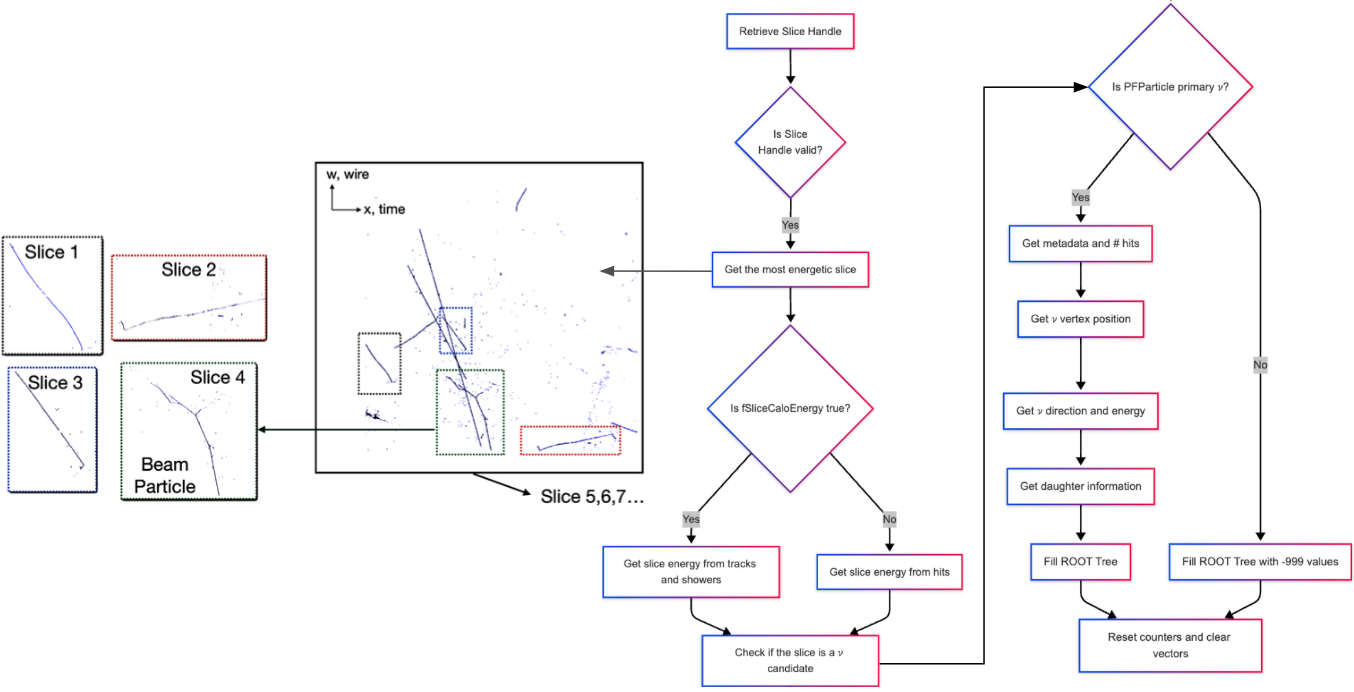
\includegraphics[width=1\linewidth]{sections/analysis/validation/logic_flowchart.png}
    \caption{Algorithm logic followed by the LArSoft analyzers employed to select reconstructed neutrino data. The concept of a Pandora slice is also illustrated on the left.}
    \label{fig:logic_flowchart}
\end{figure}

\begin{figure}[!h]
    \centering
    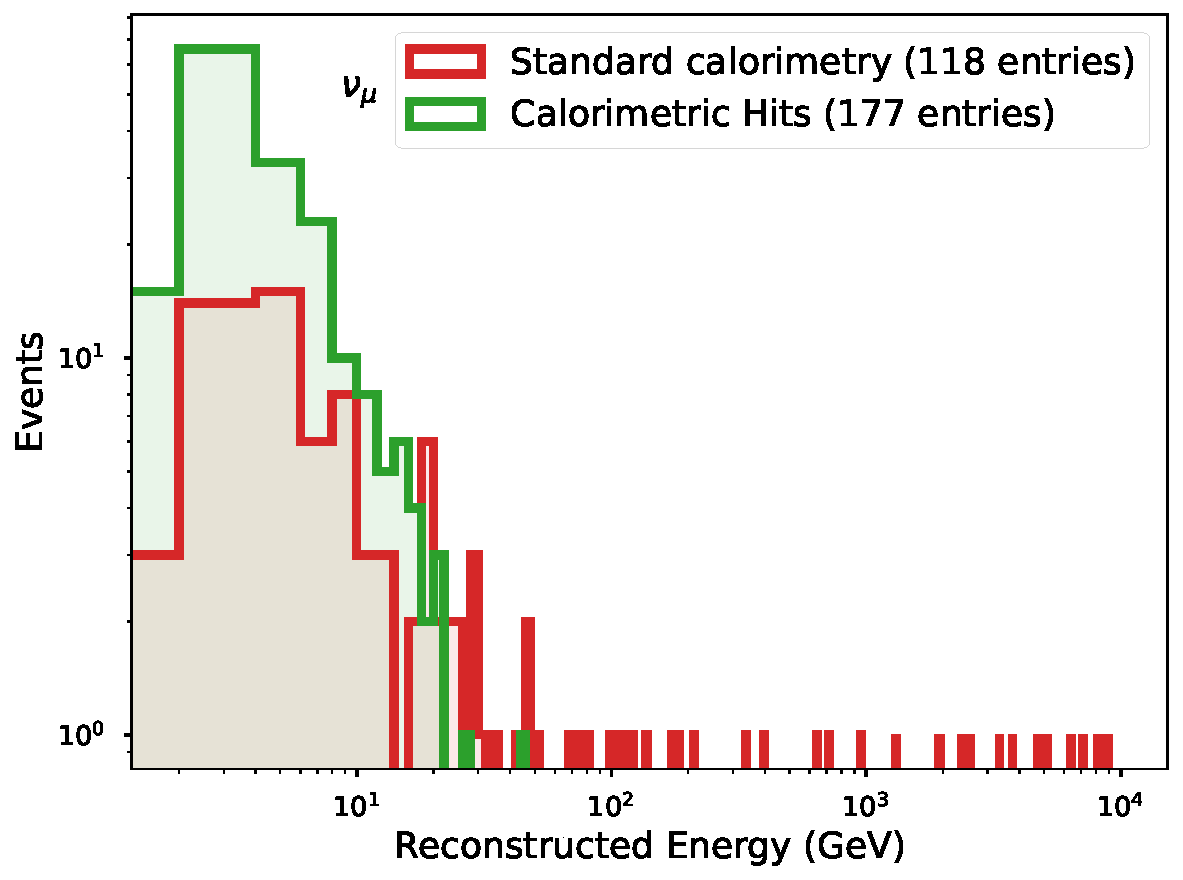
\includegraphics[width=0.75\linewidth]{sections/analysis/validation/validation_energy_methods.pdf}
    \caption{Reconstructed visible energy spectrum of neutrino candidates identified by each energy reconstruction algorithm: standard calorimetry module in red and the technique employed for atmospheric neutrino studies in green.}
    \label{fig:validation_energy_reco_methods}
\end{figure}

Next, the reconstructed neutrino information obtained with both analyzers was compared. As shown in Figure \ref{fig:validation_energy}, the reconstructed visible energy spectra for both neutrino flavors are in complete agreement. The same agreement is evident for the direction distribution of the reconstructed neutrinos from the muon-flavor set, as shown in Figure \ref{fig:validation_direction}. The same agreement is observed for the electron-flavor set.

\begin{figure}[!h]
    \centering
    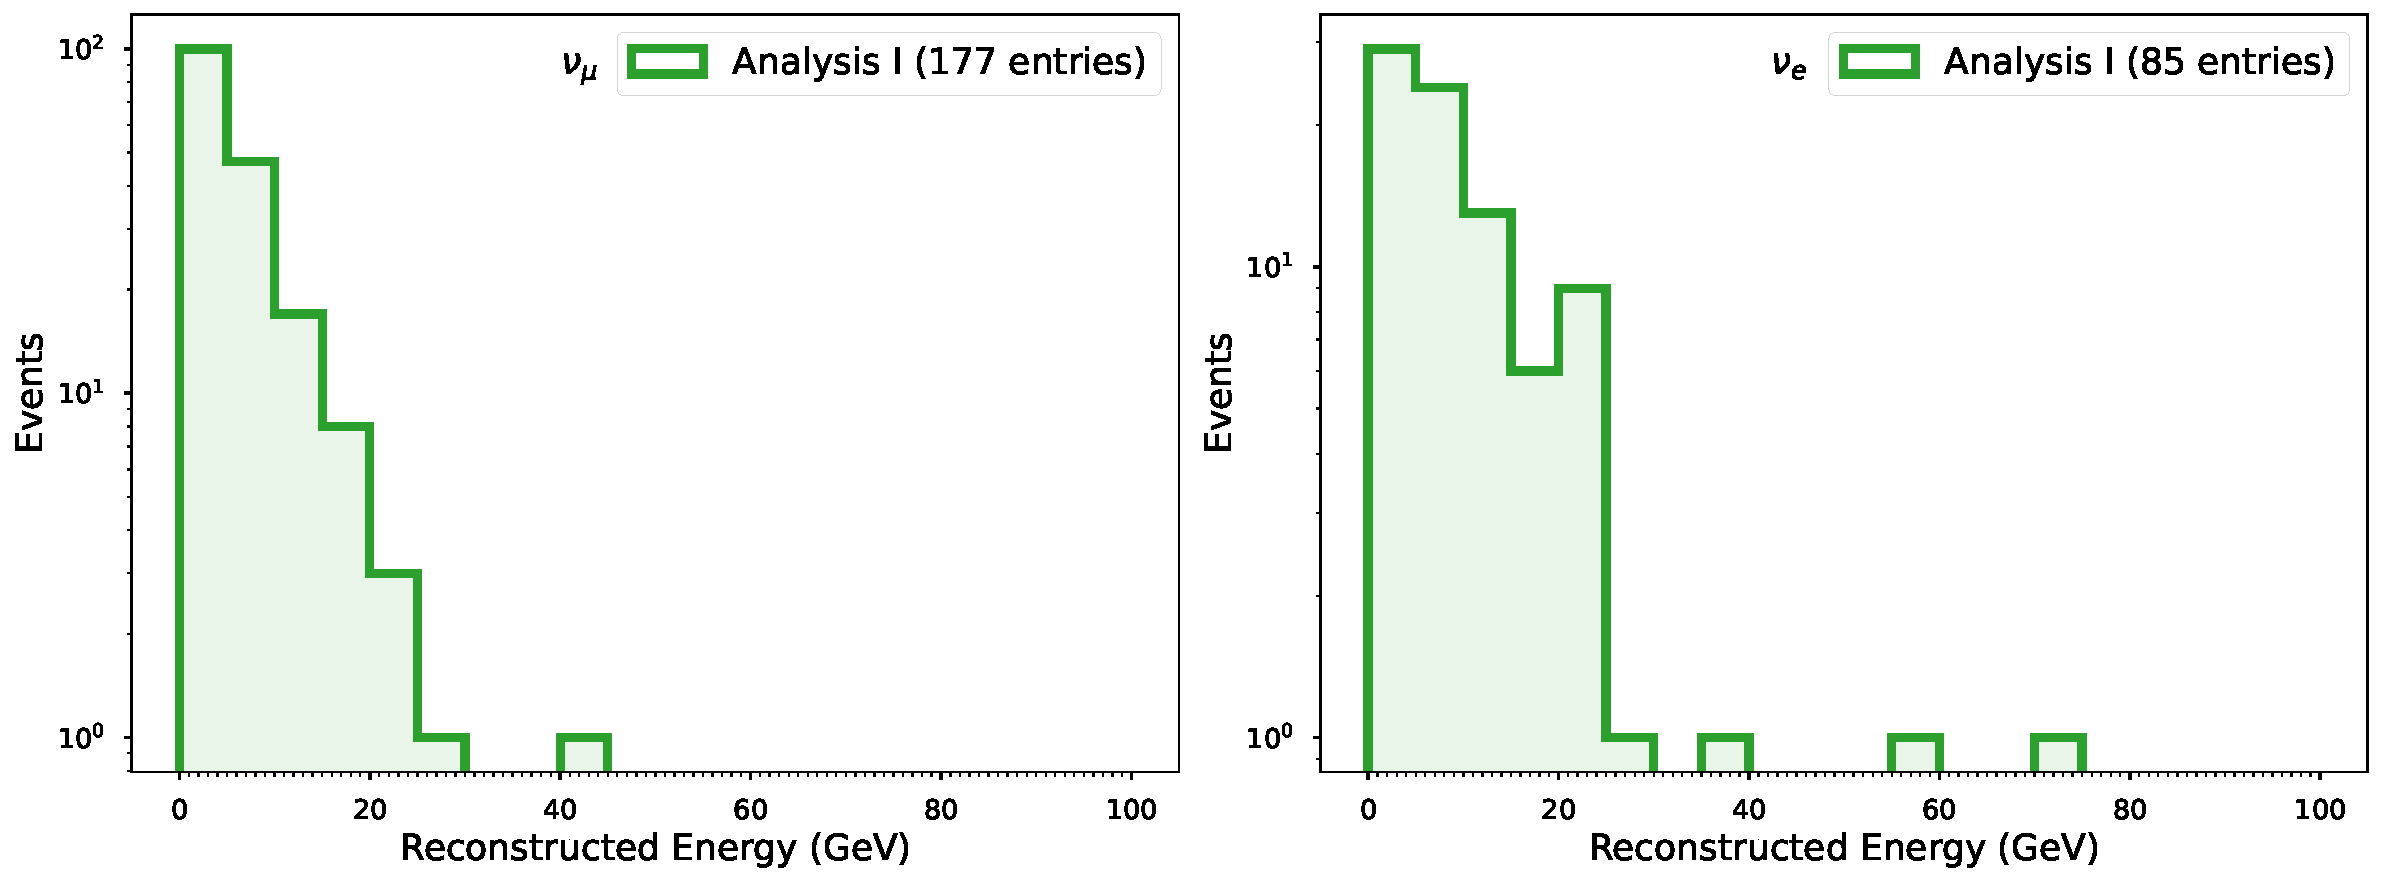
\includegraphics[width=1\linewidth]{sections/analysis/validation/new_recoEnergy_comparison.pdf}
    \caption{Reconstructed energy spectra of Monte Carlo muon neutrinos (left) and electron neutrinos (right).}
    \label{fig:validation_energy}
\end{figure}

\begin{figure}[!h]
    \centering
    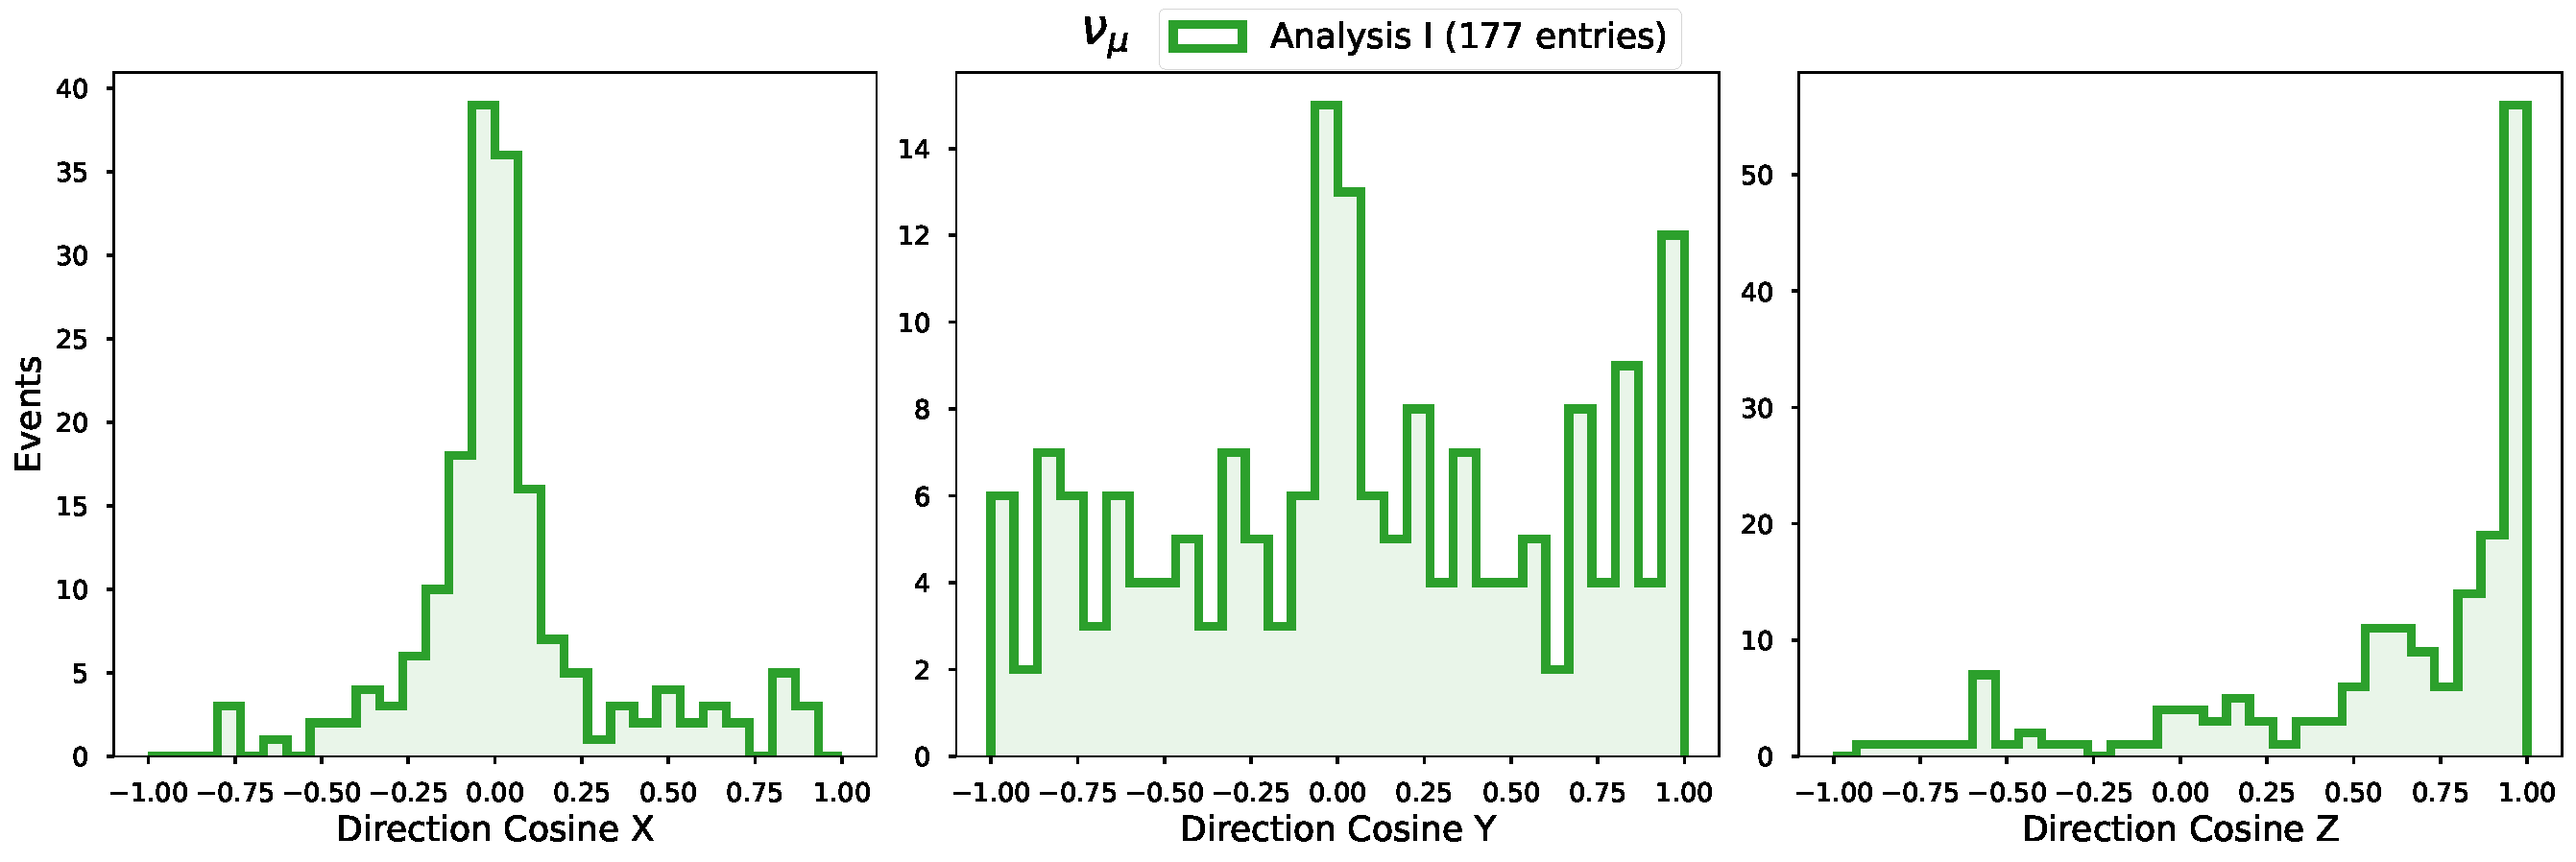
\includegraphics[width=1\linewidth]{sections/analysis/validation/new_numu_direction.pdf}
    \caption{Reconstructed direction distribution of simulated muon neutrinos in PD-HD.}
    \label{fig:validation_direction}
\end{figure}

\subsection{Variable Definition} \label{chap:Analyzer}
The information used for this analysis can be categorized into two main groups based on its source: information obtained from Pandora objects and computed independently from 2D hits. The initial phase of the Pandora-based analysis involves iterating through all accessible slices to identify the most energetic one, as neutrino events exhibit significantly higher energy levels compared to the average cosmic background. The slice energy, as discussed in the previous section, is computed using a hit-based algorithm originally developed for atmospheric neutrino events in DUNE. 

Once the slice is selected, the algorithm loops over the Particle Flow Particles (PFPs) associated with it. If a particle is labeled as a neutrino by Pandora, different variables are stored for further selection:
\begin{itemize}
    \item \textbf{Vertex position}: The vertex position associated with the neutrino interaction is saved in three variables representing the X, Y, and Z coordinates. The vertex position in the X-direction is also retrieved, but it depends on the $t_0$ of the interaction, which is provided by the Photon Detection System (PDS). Since no light information was saved during the runs, this is reconstructed using a perfect estimate, namely $t_0 = 0$, which represents the hypothetical beginning of the PDS event trigger window and cannot be trusted for events in real data.
    \item \textbf{Total direction}: Each PFP is associated with a track or shower object with a reconstructed direction. The analyzer computes the average direction over all particles associated with the neutrino interaction. This estimate is not the correct sum of the momenta of the outgoing particles because the outgoing muon often escapes the detector, leading to incomplete information; therefore, the stored direction is currently the average of the unit vectors representing the direction of each individual particle. 
    \item \textbf{Number of daughter particles}: The number of daughter particles associated with the primary neutrino PFP is saved. 
\end{itemize}



The rest of the stored variables are tailor-made using the 2D hits and, in some cases, in conjunction with information stored in Pandora objects. First, the direction of the full event is computed using a hit-based algorithm developed for atmospheric studies \cite{DUNE:2026yly}, and the result is stored for further analyses. %\footnote{\href{https://docs.dunescience.org/cgi-bin/sso/ShowDocument?docid=34618&version=3}{DocDB-34618}}.

To identify different shapes of possible showers, we need to analyze their overall shape in the Z direction, along the beam. First, the space after the vertex Z position is segmented into 10 cm bins. For each bin, the total charge from the collection plane hits is summed for the slice with the highest energy. To eliminate events from slicing failures, we calculate the Region of Interest (ROI) separately from the collection hits. The ROI represents the area in the XZ plane, respectively the drift and the anode direction, that contains the highest energy deposition. This area should correspond to the interaction that triggered the event.

First, two histograms of the charge distribution over time are generated, one for each half of the detector, which is split at the cathode. Each histogram uses 100 bins, and every hit is weighted by its detected charge. Only the half whose histogram contains the highest single-bin value is considered from this point on.
Next, the time region of interest (ROI) is defined. Starting from the peak, its edges are extended outward until the bin value falls below 20\% of the peak value; this range sets the time ROI.
Finally, the ROI in the Z direction is determined. A histogram of the Z positions of the hits is generated, again weighting each hit by its charge, but including only those hits that fall within the time ROI defined above.
The ROI is determined by adjusting the edges from the peak bin until the bin value falls below 20$\%$ of the maximum (Figure \ref{fig:ROI_scheme}). Finally, the starting and ending points of the ROI are saved for both time and Z directions for further studies.

\begin{figure}[!h]
    \centering
    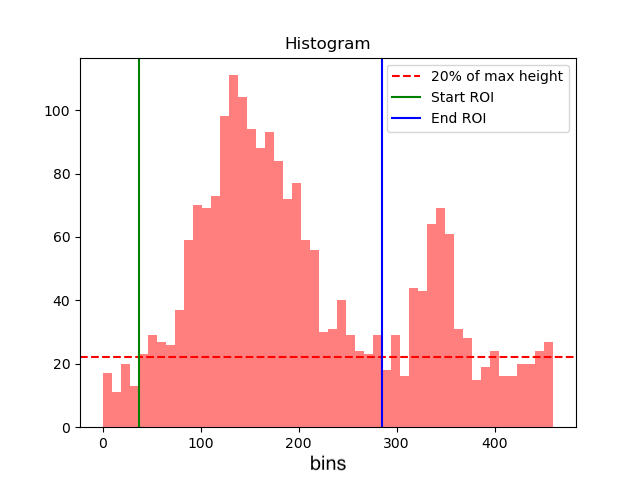
\includegraphics[width=0.59\linewidth]{sections/analysis/ROI_histogram.png}
    \caption{Representation of the ROI finding given a generic histogram. From the highest peak, the ROI borders are shifted until the counts go lower than 20\% of the maximum bin height.}
    \label{fig:ROI_scheme}
\end{figure}


\begin{figure}[!h]
    \centering
    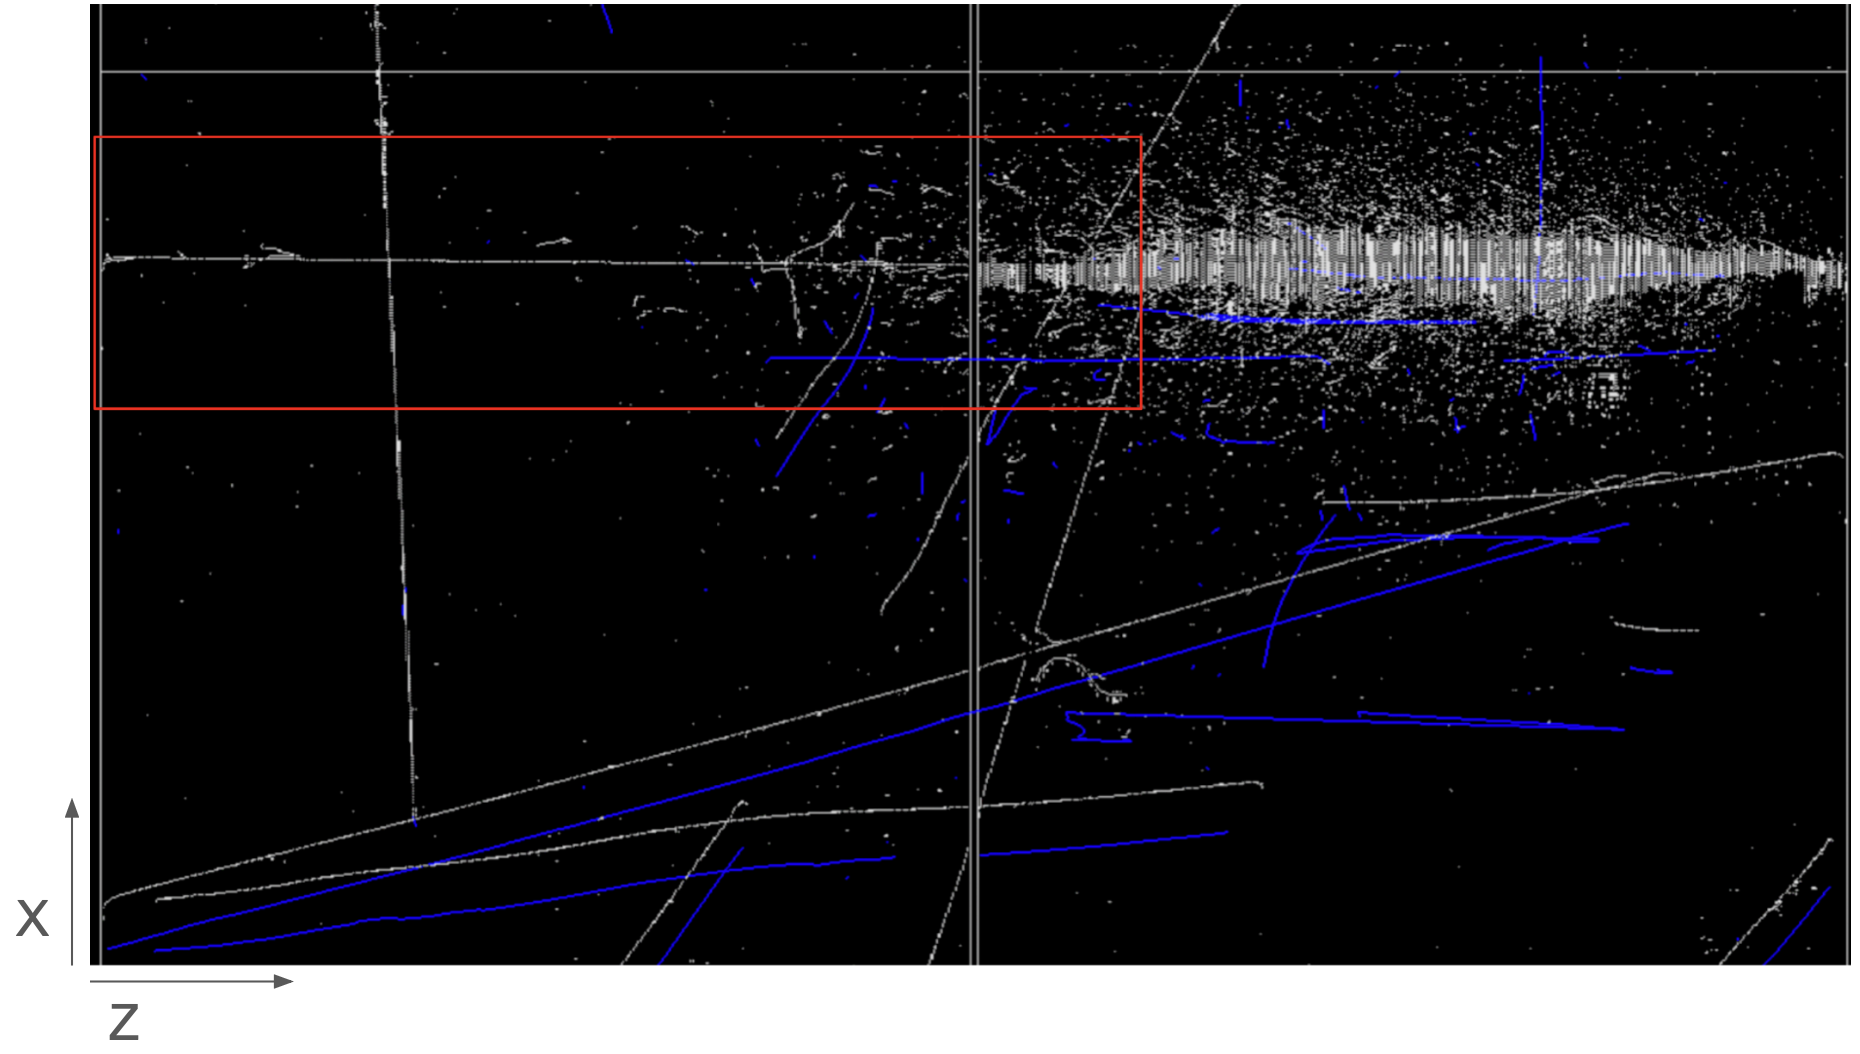
\includegraphics[width=0.59\linewidth]{sections/analysis/Selection/Failing_track.png}
    \caption{Event display of a cosmic event within PD-HD. Each gray dot represents a hit, while the blue lines correspond to the track objects from Pandora. Within the red square there is a clear track in the data which is completely lost by Pandora, leading to a poor reconstruction of the whole event.}
    \label{fig:failing_track}
\end{figure}

The topology of neutrino events presents a clear vertex inside the detector without any track connected to it before the interaction vertex. In contrast, the vast majority of cosmic events are caused by charged particles entering the detector and showering, thus presenting a track before the main shower. 
Because of the complexity of events in ProtoDUNE, it can happen that some tracks are missed in the reconstruction (or not associated with the corresponding shower), and the shower is reconstructed as a neutrino while it is actually a cosmic event (Figure~\ref{fig:failing_track}).
\begin{figure}[!h]
    \centering
    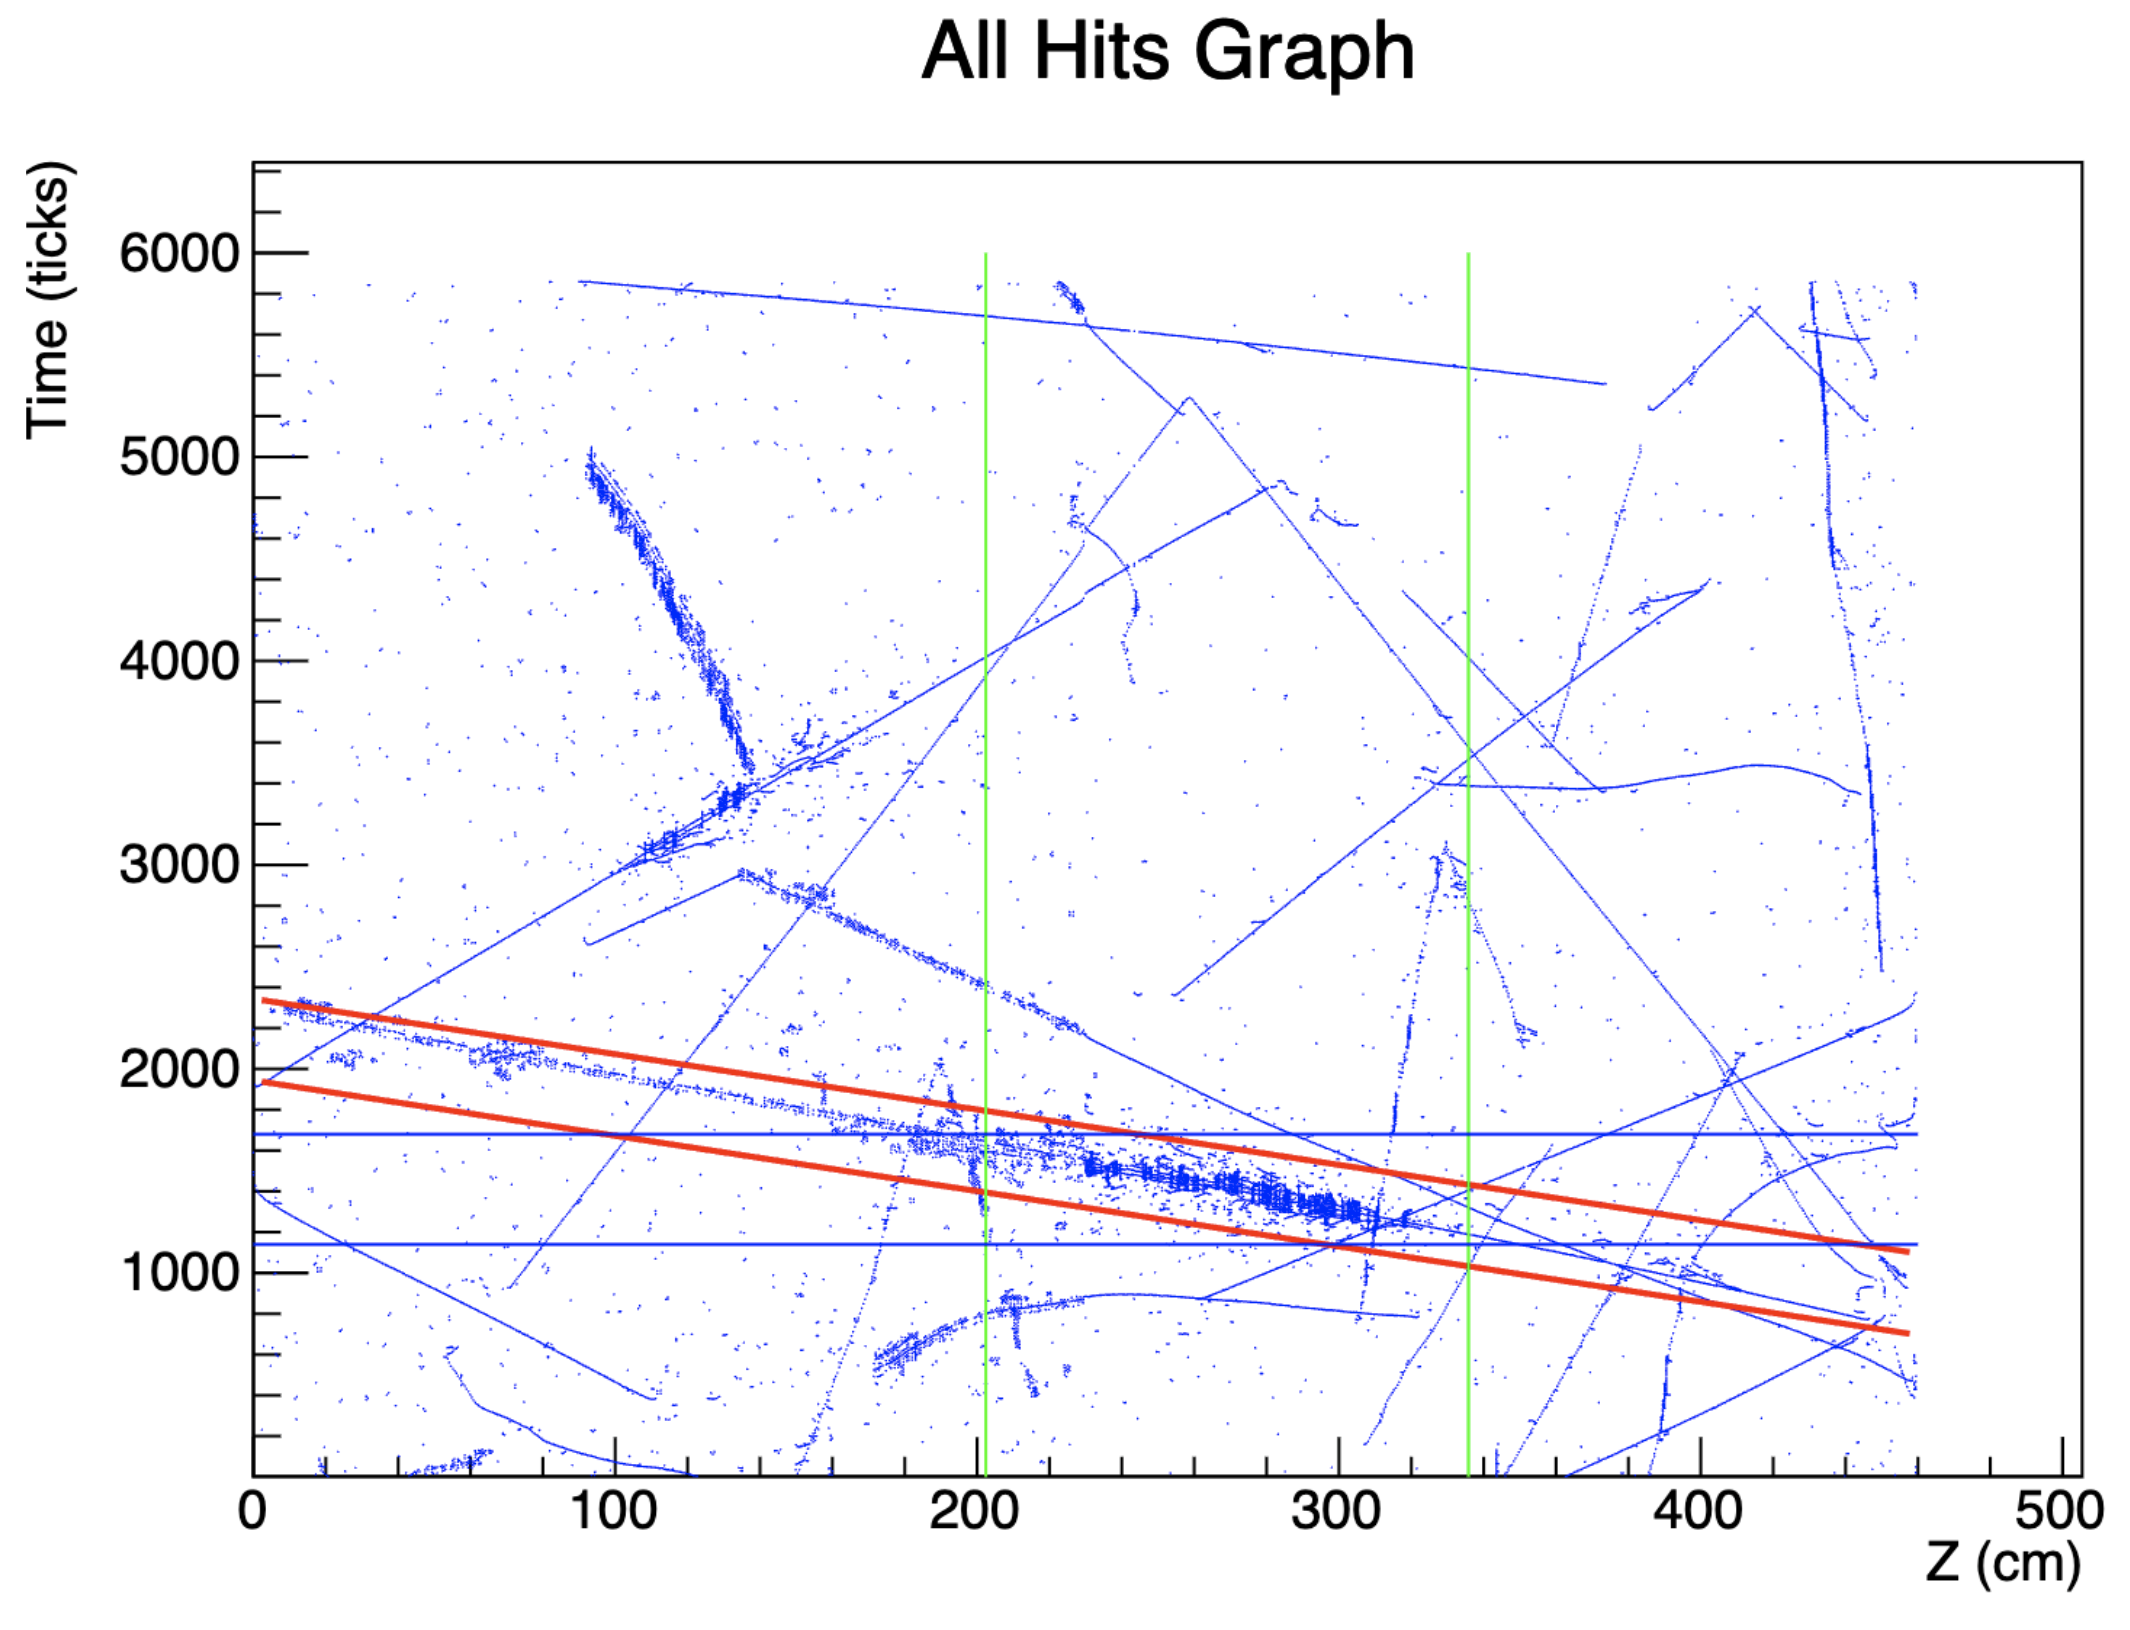
\includegraphics[width=0.59\linewidth]{sections/analysis/Selection/track_hits.png}
    \caption{Event display where each blue dot is a hit, the green vertical lines indicate the ROI in the Z coordinate, the blue horizontal lines indicate the ROI in time, and the red lines mark the borders for the tail region.}
    \label{fig:track_region}
\end{figure}
To overcome this situation, the idea is to measure the length of the hypothetical \textit{tail} before the vertex, projected onto the Z direction. To do so, the first step is to estimate the region where the tail would be if present, computed by fitting a line through the hits inside the ROI, weighting the hits by charge. The region is selected by adding and subtracting a fixed offset of 200 TPC ticks to the fitted line (Figure~\ref{fig:track_region}). 

The length is determined by counting the contiguous channels, beginning from the start of the Z ROI and moving backward, that contain at least one hit within the region. A tolerance of 1.5 cm (equivalent to three channels) is applied to correct for possible missing hits or underperforming wires. 
This method can return length values greater than zero even for real neutrinos without any track before the vertex because of pile-up, but there is a clear separation between pile-up and cosmic events with a track physically related to the shower (more in Sec.\ref{sec:EvSelection}).

\subsection{Event Selection} \label{sec:EvSelection}

\begin{table}[htbp]
\centering
\resizebox{\textwidth}{!}{%
\begin{tabular}{lcccc}
\hline
Cut & Signal Events & Bkg Events & Efficiency & Purity \\
\hline
Initial & 23.19 $\pm$ 0.23 & 2064.42 $\pm$ 6.80 &  & 1.11\% \\
Neutrino PFParticle in slice & 18.37 $\pm$ 0.21 & 1954.79 $\pm$ 6.61 &  & 0.93\% \\
Vertex fiducial volume & 16.45 $\pm$ 0.19 & 1144.34 $\pm$ 5.06 & 100.00\% & 1.42\% \\
N daughter particles & 12.52 $\pm$ 0.17 & 568.02 $\pm$ 3.57 & 76.11\% & 2.16\% \\
Max $\cos(\theta_{\mathrm{beam}})$ & 8.12 $\pm$ 0.14 & 54.47 $\pm$ 1.10 & 49.36\% & 12.97\% \\
Cut on $C_{0-10}$ & 6.99 $\pm$ 0.13 & 22.09 $\pm$ 0.70 & 42.49\% & 24.04\% \\
Cut on $C_{40-50}$ & 6.00 $\pm$ 0.12 & 15.91 $\pm$ 0.60 & 36.47\% & 27.38\% \\
Cut on $C_{140-150}$ & 4.83 $\pm$ 0.11 & 8.62 $\pm$ 0.44 & 29.36\% & 35.91\% \\
ROI Z size & 4.67 $\pm$ 0.10 & 5.37 $\pm$ 0.35 & 28.39\% & 46.51\% \\
ROI Z close to vertex & 3.73 $\pm$ 0.09 & 2.08 $\pm$ 0.22 & 22.67\% & 64.20\% \\
Tail Length Density & 2.85 $\pm$ 0.08 & 0.67 $\pm$ 0.12 & 17.33\% & 80.97\% \\
\hline
\end{tabular}
}
\caption{Expected number of events during all steps of the selection, weighted to one hour of beam-on data, with the cumulative signal purity after each cut. The cumulative signal efficiency is computed relative to the number of neutrinos inside the fiducial volume (100\% at the ``Vertex fiducial volume'' row); it is left blank for the two preceding, pre-fiducial-volume stages.}
\label{tab:filter_evolution}
\end{table}

Before any cut is applied, the expected number of neutrino events in the data is negligible compared to the background, as illustrated in Table~\ref{tab:filter_evolution}. Consequently, it is crucial to maximize the use of available information. Each cut is optimized using Monte Carlo neutrinos, which represent the signal, and beam-off data, which represent the background, as explained in section \ref{chap:montecarlo_samples}.

Table~\ref{tab:filter_evolution} shows the effect of the sequential cuts on the initial dataset, applied in the order described below.

The first requirement is that Pandora labels the most energetic slice as containing a neutrino interaction, as described in Section~\ref{chap:anaValidation}; events without a reconstructed neutrino candidate in that slice are discarded at this stage (Table~\ref{tab:filter_evolution}).

To remove events originating outside the cryostat, a fiducial volume cut on the vertex reconstructed by Pandora is applied. To remove events from above or upstream, cuts are placed at $V_y \leq 550$~cm (Figure~\ref{fig:vertexY}) and $V_z \geq 20$~cm (Figure~\ref{fig:vertexZ}), respectively.

High-energy neutrino events are expected to produce large showers with many daughter particles. If Pandora identifies a neutrino interaction, it associates a virtual neutrino mother with all the reconstructed particles related to the event with a mother-daughter hierarchy. Then, a cut on the number of neutrino daughter particles is set at $N_{\text{daughters}} \geq 6$ to enhance the signal-to-background ratio (Figure~\ref{fig:nPFPs}).

\begin{figure}[!h]
    \centering
    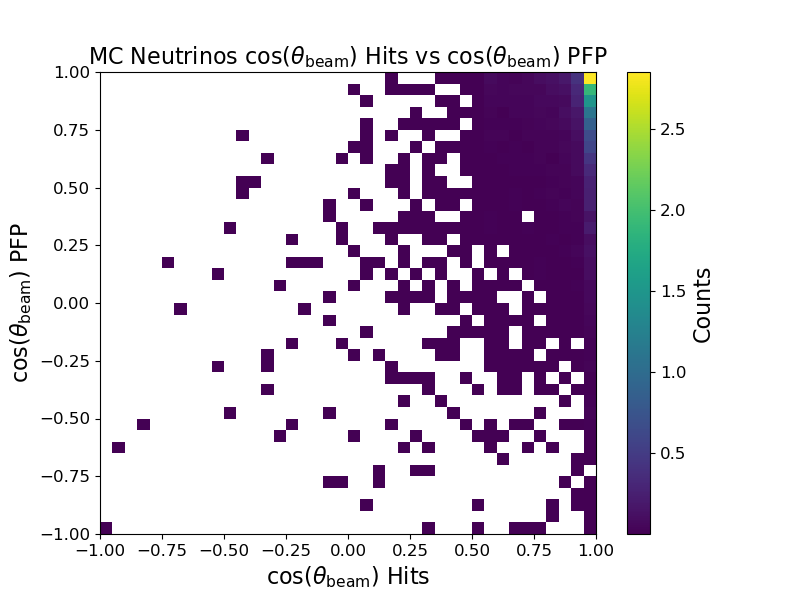
\includegraphics[width=0.59\linewidth]{sections/plots/version_2/selection_cuts/all_cuts_False/sig_directionZ_vs_directionZ2.png}
    \caption{2D histogram showing the $\cos(\theta_{\mathrm{beam}})$ computed with two different reconstruction methods.}
    \label{fig:z1_vs_z2}
\end{figure}
\begin{figure}[!h]
    \centering
    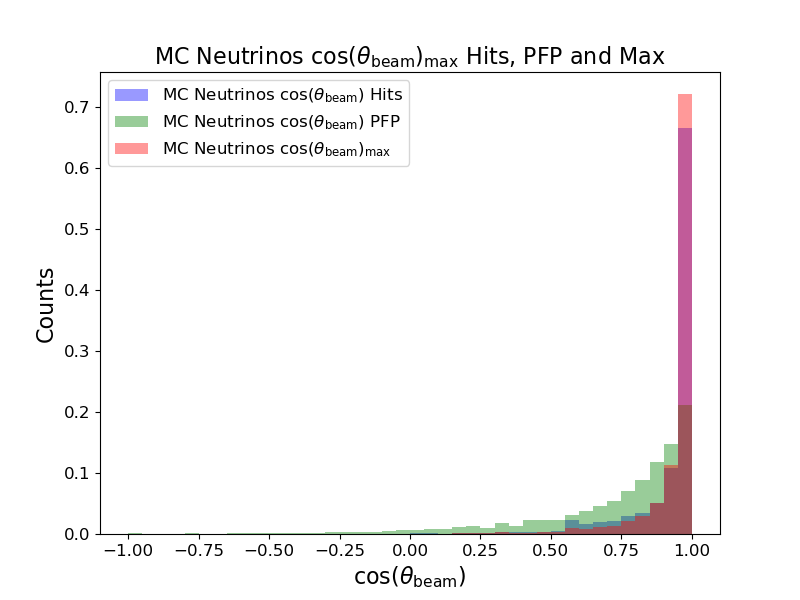
\includegraphics[width=0.49\linewidth]{sections/plots/version_2/selection_cuts/all_cuts_False/sig_direction_histograms.png}
    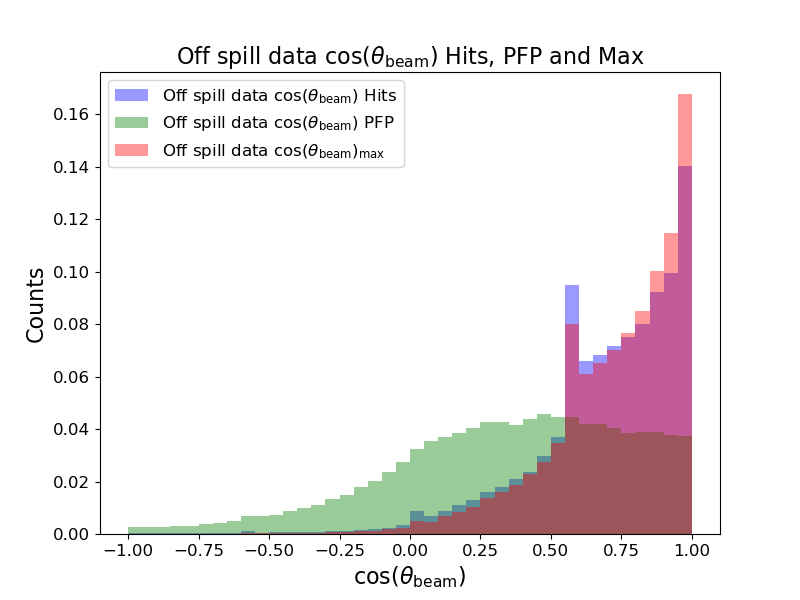
\includegraphics[width=0.49\linewidth]{sections/plots/version_2/selection_cuts/all_cuts_False/bkg_direction_histograms.png}
    \caption{1D histograms showing the $\cos(\theta_{\mathrm{beam}})$ computed with two different reconstruction methods and the maximum value between the two for the Monte Carlo neutrinos (left) and the spill-off data (right).}
    \label{fig:z1_vs_z2_1d}
\end{figure}
% The key feature distinguishing cosmic events from neutrinos is the shower direction, reflected by the fact that this variable produces the most significant cut.
The primary distinguishing factor between cosmic events and neutrinos is their direction of travel. Neutrinos originate from a single point along the beam and travel parallel to the Z-axis, while cosmic rays arrive at Earth from all directions randomly. Since ProtoDUNE is located in a pit, the vast majority of the cosmic rays detected by the detector come with a significant component parallel to the Y-axis.
% To mitigate differences between reconstruction algorithms developed for different purposes and potentially unreliable for this kind of event, we take the maximum value of $\cos(\theta_{\mathrm{beam}})$ computed with both the hits-based and Pandora-based algorithms.
The results of the two functions used to compute the event direction (see Sec.\ref{chap:Analyzer}) are not perfectly correlated (Figure~\ref{fig:z1_vs_z2}), indicating that there is room for improvement in the final result by utilizing both methods instead of relying solely on one.
A new variable is introduced as the maximum value of $\cos(\theta_{\mathrm{beam}})$ obtained from the two results (Figure \ref{fig:z1_vs_z2_1d}), leveraging the knowledge about the true direction of the neutrino beam. This new variable helps in recovering more neutrinos in the selection process, without a substantial increase in the number of cosmic rays that enter the analysis.

The cut on this variable is set at $\cos(\theta_{\mathrm{beam}})_{_\text{max}} > 0.97$ (Figure~\ref{fig:maxZ}) and reduces the number of background events substantially (Table \ref{tab:filter_evolution}).

From the $\cos(\theta_{\mathrm{beam}})_{\text{max}}$ distribution (Figure~\ref{fig:maxZ}), many cosmic events appear to travel horizontally along the beam direction, though this is often not the case. This effect arises because Pandora is tuned to identify horizontal neutrinos without significant background, and, combined with imperfect Y-coordinate reconstruction, it sometimes misplaces the vertex of a downward shower, reconstructing a vertical event as horizontal.
To mitigate this, the energy deposition profile in the beam direction is examined. The space after the vertex is divided into 10 cm bins along Z, and the charge per bin is stored as described in section \ref{chap:Analyzer}.
Cuts on all bins proved redundant; therefore, cuts are applied only in the 0–10~cm, 40–50~cm, and 140–150~cm bins after the vertex, defined as
$$
C_{0-10}>3000 \text{~ADC}, \quad C_{40-50}>10000\text{~ADC}, \quad C_{140-150}>3000\text{~ADC}.
$$

The ROI along the Z-axis is used to select the events where the neutrino showers develop horizontally, as expected. Consequently, a cut on the ROI is applied, and only events with a sufficiently large ROI size along the Z-axis are selected by requiring $L_{\text{ROI}} > 70$~cm (Figure~\ref{fig:ROIsize}).

The reconstructed neutrino vertex position is a central information from which the hits-based direction algorithm reconstructs the orientation of the event, but, as noted, it is not always reliable.
The ROI position computed from low-level hits (section \ref{chap:Analyzer}) is an independent indication about the position of the event in the detector, and can offer a double check for the vertex position. Therefore, to reject events with unrealistic vertex positions, we compare the vertex position along the Z-axis with the ROI start position computed from low-level hits (section \ref{chap:Analyzer}).
Events with $\lvert Z_{\text{vertex}} - Z_{\text{ROI}} \rvert > 20$~cm are removed (Figure~\ref{fig:ROIdistance}).

During development, it was observed that many particles identified as neutrinos had a muon track upstream of the related shower, indicating the shower was induced by cosmic events. Using the low level hit objects ensures a reliable way of removing such topologies ignoring any possible malfunctioning of the more complicated tools.
Finally, using the track length variable described in section \ref{chap:Analyzer}, we apply a cut on the ratio between the track length and the distance of the ROI start position from the upstream wall (Figure~\ref{fig:tailDensity}), defined as $$\text{Tail density} = \frac{L_{\text{tail}}}{L_{\text{tot}}} < 0.2~~~~~.$$




